\documentclass[]{article}

\usepackage{graphicx}
\usepackage{subcaption}

%opening
\title{Project Documentation for \\Mathematics of Neural Networks}
\author{Johann Kipping}

\begin{document}

\maketitle

\begin{abstract}
The aim of this project is to test the learned things in the first half of the lecture series on Neural Networks on the example of the Fashion-MNIST Dataset\\
\\
Things that could be done on Fashion-MNIST
\begin{itemize}
	\item Hyperparameter search
	\item Activation functions
	\item Initialization
	\item Optimizers
	\item Regularization (Overfitting?) + Generality
	\item FFT/im2col/Winograd
	\item Attribution
	\item Feature Visualization
	\item Adversarial Attacks
	\item Going deep?
\end{itemize}
\end{abstract}

\section*{0\quad Getting TF to run with a GPU with CUDA CC of 3.0}
As this is a documentation of work it will be mentioned that a significant amount of time needed for the setup of computations was put into getting tensorflow to compute on the available GPU (Geforce 660 Ti). The major obstacle was the fact that this particular GPU has a \textit{CUDA compute capability} of 3.0. The least tensorflow supports as of now is 3.5. This lead to the necessity of \textbf{downgrading to tensorflow version 1.12}. This might impede the ability for coverage of advanced topics.

\section{Idea collection and planning}
\label{ideas}
This chapter aims to collect ideas to most of the topics that were discussed in the lecture and continues to formulate a plan on how to tackle them in this project work.\\
\\
Loss functions used is categorical cross entropy. Why not Mean squared or something else\\
\\
\textbf{Hyperparameters:}\\
Idea: Try several choices of hyperparameters to get a feel for the effects. Do this in a grid-like fashion.\\
\\
\textbf{Activation functions / network structure}\\
Idea: Test small network structures (fast trainable) for effect of structural changes and different choices of activation functions using knowledge from the lecture and Exercise 4 from sheet 6 as starting point for network evaluation.\\
\\
\textbf{Initialization}\\
Idea: Verify the validity of the three approaches discussed in the lecture. (Zero/Random/Known data)\\
\\
\textbf{Optimizers}\\
Idea: Use Adam for all computations to reduce complexity of project as it incorporates other approaches.\\
\\
\textbf{Regularization (Overfitting?) + Generality}\\
Idea: Test for overfitting and generalization with own pictures (for fun). Maybe try regularization if poor performance is observed.\\
\\
\textbf{FFT/im2col/Winograd}\\
Idea: Let tensorflow decide on the usage of different approaches as insight was achieved in the exercises and modifications are not cheap.\\
\\
\textbf{Attribution/Feature Visualization}\\
Idea: Visualize the computed nets feature maps by using Saliency maps and grad-Cam. Try out deconvolution/guided backpropagation (DeconvNet) if possible! Relu has to be used! \\
\\

Progress will be documented with screenshots of the console and explanation. Graphs will be used.

\section{Getting to know Neural Networks}
This section will describe the first set of investigative experiments. Mainly regarding stuff of the first couple of lectures its main aim is to allow to get an understanding and feeling for the behavior of Neural Networks.

\subsection{Starting out}
As a starting point the network structure from Exercise 4 of sheet 6 was chosen to allow further investigation. As described in section \ref{ideas} Adam was be used as the optimizer throughout this section in order to reduce complexity.

\subsection{Initialization experiments}
The methods for initializations are to be tested in this section:
\begin{itemize}
	\item zero
	\item known data
	\item random
\end{itemize}
As mentioned before the net structure used for this will be structure from Exercise 4 of sheet 6.\\
The random initialization will be employed before the known data approach as the results from the random initialization will be used as the known data.
\subsubsection{Zero initialization}
As expected little to no improvement can be seen from training.
\subsubsection{Random initialization}
The baseline performance seen in the exercise. Uniform he initializer was used.
\subsubsection{Known data initialization}
This method allow the last two dense layers for classification to be further trained. This improved the networks performance for the training data, not for the test data

\begin{figure}[h!]
	\begin{subfigure}{.3\textwidth}
		\centering
		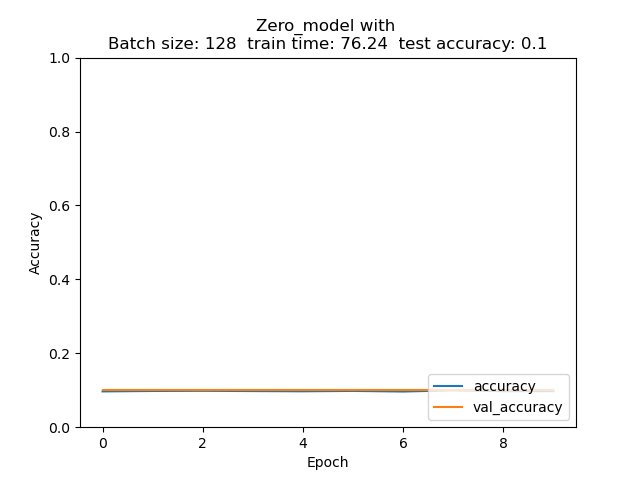
\includegraphics[width=\linewidth]{../img_1_1_init/acc_plot_Zero_model.png}
		\caption{1a}
		\label{fig:sfig1}
	\end{subfigure}%
	\begin{subfigure}{.3\textwidth}
		\centering
		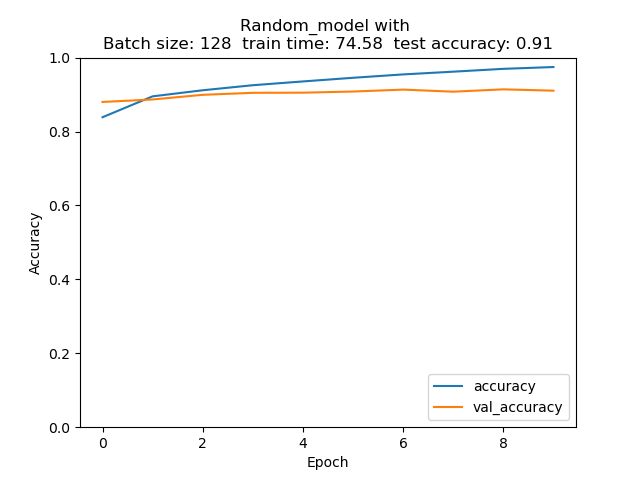
\includegraphics[width=\linewidth]{../img_1_1_init/acc_plot_Random_model}
		\caption{1b}
		\label{fig:sfig2}
	\end{subfigure}
	\begin{subfigure}{.3\textwidth}
		\centering
		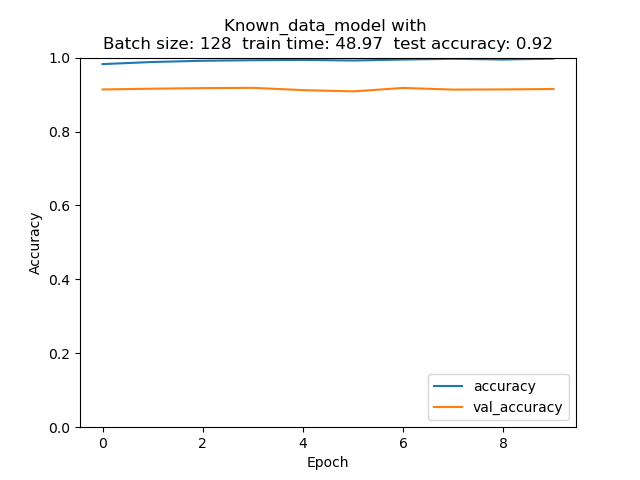
\includegraphics[width=\linewidth]{../img_1_1_init/acc_plot_Known_data_model}
		\caption{1b}
		\label{fig:sfig2}
	\end{subfigure}
	\caption{plots of....}
	\label{fig:fig}
\end{figure}

\subsection{Network structure}
\subsection{Hyperparameters}


\section{Regularization and Attribution}
Check for generality and attribute in the same step by using an image from the test set and an image that was taken by me\\
\\
Using gradient tape -> saliency map\\
Global average pooling -> class activation map\\
Grad-CAM! am ehesten

\end{document}
